%! TeX program = xelatex
\documentclass[a4paper]{scrartcl}
\usepackage{polyglossia}
\setdefaultlanguage{english}
\usepackage{amsmath}
\usepackage{amsfonts}
\usepackage{amssymb}
\usepackage{graphicx}
\usepackage{fullpage}
\usepackage{tikz}
\usetikzlibrary{fadings}
\usetikzlibrary{patterns}
\usetikzlibrary{shadows.blur}
\usetikzlibrary{shapes}
\begin {document}
\section{Anisotropic Fresnel coefficients}

\tikzset{every picture/.style={line width=0.75pt}} %set default line width to 0.75pt

\begin{figure}[b!]
\centering
\begin{tikzpicture}[x=0.75pt,y=0.75pt,yscale=-1,xscale=1]
      \draw (20,174) -- (425,174);
      \draw [shift={(428.41,174.07)}, rotate = 180][fill={rgb, 255:red, 0; green, 0; blue, 0}][line width=0.08][draw opacity=0]
            (8.93,-4.29) -- (0,0) -- (8.93,4.29) -- cycle;
      \draw    (213,14) -- (213,360);
      \draw [shift={(213,11.29)}, rotate = 90][fill={rgb, 255:red, 0; green, 0; blue, 0 }][line width=0.08][draw opacity=0]
            (8.93,-4.29) -- (0,0) -- (8.93,4.29) -- cycle;
      \draw (79,174) .. controls (79,100) and (360,100) .. (360,174);
      \draw (213,174) -- (110,332);
      \draw (332,63) -- (213,174);
      \draw [shift={(335,61)}, rotate = 137.28][fill={rgb, 255:red, 0; green, 0; blue, 0}][line width=0.08][draw opacity=0]
            (8.93,-4.29) -- (0,0) -- (8.93,4.29) -- cycle;
      \draw [line width=1.5]    (213,174) -- (266,126);
      \draw [shift={(268,124)}, rotate = 497.76][color={rgb, 255:red, 0; green, 0; blue, 0}][line width=1.5]
            (14.21,-4.28) .. controls (9.04,-1.82) and (4.3,-0.39) .. (0,0) .. controls (4.3,0.39) and (9.04,1.82) .. (14.21,4.28);
      \draw [line width=1.5]    (110,332) -- (164,250);
      \draw [shift={(165.57,248.21)}, rotate = 483.07][color={rgb, 255:red, 0; green, 0; blue, 0}][line width=1.5]
            (14.21,-4.28) .. controls (9.04,-1.82) and (4.3,-0.39) .. (0,0) .. controls (4.3,0.39) and (9.04,1.82) .. (14.21,4.28);
      \draw (165,248) -- (203,270);
      \draw [shift={(205,271)}, rotate = 210.33][color={rgb, 255:red, 0; green, 0; blue, 0}][line width=0.75]
            (10.93,-3.29) .. controls (6.95,-1.4) and (3.31,-0.3) .. (0,0) .. controls (3.31,0.3) and (6.95,1.4) .. (10.93,3.29);
      \draw (268,124) -- (294,145);
      \draw [shift={(295.28,146.61)}, rotate = 219.95][color={rgb, 255:red, 0; green, 0; blue, 0}][line width=0.75]
            (10.93,-3.29) .. controls (6.95,-1.4) and (3.31,-0.3) .. (0,0) .. controls (3.31,0.3) and (6.95,1.4) .. (10.93,3.29);
      \draw (213.29,174.07) -- (316.08,332.76);
      \draw [line width=1.5] (267,257) -- (213,175);
      \draw [shift={(268.36,259.49)}, rotate = 236.93][color={rgb, 255:red, 0; green, 0; blue, 0}][line width=1.5]
            (14.21,-4.28) .. controls (9.04,-1.82) and (4.3,-0.39) .. (0,0) .. controls (4.3,0.39) and (9.04,1.82) .. (14.21,4.28);
      \draw (268,260) -- (230,282);
      \draw [shift={(228.53,282.76)}, rotate = 329.7][color={rgb, 255:red, 0; green, 0; blue, 0}][line width=0.75]
            (10.93,-3.29) .. controls (6.95,-1.4) and (3.31,-0.3) .. (0,0) .. controls (3.31,0.3) and (6.95,1.4) .. (10.93,3.29);
      \draw (92,62) -- (213,175);
      \draw [line width=1.5] (138,104) -- (85,56);
      \draw [shift={(140,105.83)}, rotate = 222.24][color={rgb, 255:red, 0; green, 0; blue, 0}][line width=1.5]
            (14.21,-4.28) .. controls (9.04,-1.82) and (4.3,-0.39) .. (0,0) .. controls (4.3,0.39) and (9.04,1.82) .. (14.21,4.28);
      \draw (140,106) -- (114,128);
      \draw [shift={(112.4,128.96)}, rotate = 320][color={rgb, 255:red, 0; green, 0; blue, 0}][line width=0.75]
            (10.93,-3.29) .. controls (6.95,-1.4) and (3.31,-0.3) .. (0,0) .. controls (3.31,0.3) and (6.95,1.4) .. (10.93,3.29);
      \draw (425,190) node  [font=\normalsize] [align=left] {y};
      \draw (195,12) node [anchor=north west][inner sep=0.75pt]  [font=\normalsize] [align=left] {z};
      \draw (360,110) node [anchor=north west][inner sep=0.75pt]  [font=\normalsize]  {$\dfrac{\omega ^{2}}{c^{2}}
            =\dfrac{k_{y}}{\epsilon _{\bot}} +\dfrac{k_{z}}{\epsilon _{\parallel}}$};
      \draw (297,145) node [anchor=north west][inner sep=0.75pt]  [font=\normalsize]  {$E_{2}^{+}$};
      \draw (170,270) node [anchor=north west][inner sep=0.75pt]  [font=\normalsize]  {$E_{1}^{+}$};
      \draw (115,273) node [anchor=north west][inner sep=0.75pt]  [font=\normalsize]  {$k_{1}^{+}$};
      \draw (250,140) node [anchor=north west][inner sep=0.75pt]  [font=\normalsize]  {$k_{2}^{+}$};
      \draw (245,270) node [anchor=north west][inner sep=0.75pt]  [font=\normalsize]  {$E_{1}^{-}$};
      \draw (95,105) node [anchor=north west][inner sep=0.75pt]  [font=\normalsize]  {$E_{2}^{-}$};
      \draw (110,60) node [anchor=north west][inner sep=0.75pt]  [font=\normalsize]  {$k_{2}^{-}$};
      \draw (260,217) node [anchor=north west][inner sep=0.75pt]  [font=\normalsize]  {$k_{1}^{-}$};
      \draw (360,180) node [anchor=north west][inner sep=0.75pt]  [font=\normalsize]  {$\epsilon_{\textrm{rel}}
      	,\mu_{\textrm{rel}}$};
      \draw (335,20) node [anchor=north west][inner sep=0.75pt]  [font=\normalsize]  {$\epsilon \ =\ \begin{pmatrix}
      \epsilon _{\parallel} & 0 & 0\\
      0 & \epsilon _{\parallel} & 0\\
      0 & 0 & \epsilon _{\bot}
      \end{pmatrix}$};
      \draw (195,208) node [anchor=north west][inner sep=0.75pt]  [font=\small]  {$\theta_{1}$};
      \draw (220,208) node [anchor=north west][inner sep=0.75pt]  [font=\small]  {$\theta_{1}$};
      \draw (195,140) node [anchor=north west][inner sep=0.75pt]  [font=\small]  {$\theta_{2}$};
      \draw (220,140) node [anchor=north west][inner sep=0.75pt]  [font=\small]  {$\theta_{2}$};
\end{tikzpicture}
\caption{An interface between an isotropic and anisotropic medium. Wavevectors corresponding to incident, reflected and transmitted waves are shown
on both sides of the interface. TM polarization.}
\label{Fig. 1}
\end{figure}
Let us consider an interface between an isotropic and an anisotropic medium, as shown in figure \ref{Fig. 1}. Sice we
are focusing on the case of uniaxial anisotropy (only the $\epsilon_{zz}$ component of the permittivity tensor is
different) the case of TE polarized waves is trivial, since the incident wave does not interact with the anomalous
component of the permittivity tensor. TM polarized light has only the x component of magnetic intensity field
$\mathbf{H}=(H_x,0,0)$.
Let us now consider a wavi incident on the interface from the isotropic side.
Utilizing Maxwell's equations we can connect the magnitudes of components of the electric intensity fiels with the
x-component of magetic intensity:
\begin{equation}
      \mathbf{k}_1 \times \mathbf{H}_1 = -\omega\epsilon\mathbf{E}_1
\end{equation}
\begin{equation}
      E_{1y} = \dfrac{-k_{1z} H_{1x}}{\omega \epsilon_\textrm{rel}}
\end{equation}
\begin{equation}
      E_{1z} = \dfrac{k_{1y} H_{1x}}{\omega \epsilon_\textrm{rel}}
\end{equation}
furthermore, since k-vector of the incident wave has the form
\begin{equation}
      \mathbf{k}_1^+ = (0,k_{1y}^+,k_{1z}^+)
\end{equation}
we can immediately get the y-component from the angle of incidence
\begin{equation}
      k_{1y}^+ = k_1^+ \sin(\theta_1) = \sqrt{\epsilon_\textrm{rel}}\dfrac{\omega}{c} \sin\theta_1
\end{equation}
and utilizing dispersion relation in the anisotropic medium we can get the z-component of transmitted k-vector:
\begin{equation}
      k_z =
      \sqrt{\epsilon_\parallel}\dfrac{\omega}{c}\sqrt{1-\dfrac{\epsilon_\textrm{rel}}{\epsilon_\bot}\sin^2\theta_1}
\end{equation}
because the y component of the wave vector is conserved across the interface. Now we can formulate conservation
relations for other fields:
\begin{equation}
      \mathbf{H}_1^+ + \mathbf{H}_1^- = \mathbf{H}_2^+
\end{equation}
\begin{equation}
      E_{1y}^+ + E_{1y}^- = E_{2y}^+
\end{equation}
These can be obtained by applying Maxwell's equations to the interface. In equations (7) and (8) we are considering only
the incident, reflected and transmitted waves (we are excluding the wave labeled as $\mathbf{k}_2^-$)
Now, let us apply equation (1) on the anisotropic side of the interface. Again, carefully observing, that permittivity
is a tensor, we get:
\begin{equation}
      E_{2y} = \dfrac{-k_{2z} H_{2x}}{\omega \epsilon_\parallel}
\end{equation}
\begin{equation}
      E_{2z} = \dfrac{k_{2y} H_{2x}}{\omega \epsilon_\bot}
\end{equation}
Since $\mathbf{k}_1^+ = -\mathbf{k}_1^-$ we can combine equations (2), (8) and (9) to get
\begin{equation}
\dfrac{-k_{1z}^+ H_{1x}^+}{\omega \epsilon_\textrm{rel}} + \dfrac{+k_{1z}^+ H_{1x}^-}{\omega \epsilon_\textrm{rel}} =
\dfrac{-k_{2z}^+ H_{2x}^+}{\omega \epsilon_\parallel}
\end{equation}
further applying equation (7) we obtain:
\begin{equation}
      \mathbf{H}_{2x}^+ =
      \dfrac{\dfrac{2k_{1z}^+}{\epsilon_\textrm{rel}}}{\dfrac{k_{2z}^+}{\epsilon_\parallel} +
      \dfrac{k_{1z}^+}{\epsilon_\textrm{rel}}} \mathbf{H}_{1x}^+
\end{equation}
Now let us calculate the Poynting vector
\begin{equation}
      \mathbf{S} = \mathbf{E} \times \mathbf{H}
\end{equation}
\begin{equation}
      \mathbf{S} = (0,H_x E_z, -H_x E_y)
\end{equation}
plugging in equations (2), (3), (9) and (10):
\begin{equation}
      \mathbf{S}_1^+ = \dfrac{\mathbf{H}_{1x}^{+2}}{\omega\epsilon_{\textrm{rel}}}(0,k_{1y}^+, k_{1z}^+)
\end{equation}
\begin{equation}
      \mathbf{S}_2^+ = \dfrac{\mathbf{H}_{2x}^{+2}}{\omega}(0,\dfrac{k_{2y}^+}{\epsilon_\bot},
      \dfrac{k_{2z}^+}{\epsilon_\parallel})
\end{equation}
Coefficient of transmittivity is given as
\begin{equation}
      T = \dfrac{S_{2z}^+}{S_{1z}^+} = \left| \dfrac{H_{2x}^+}{H_{1x}^+} \right| ^2 \dfrac{k_{2z}^+}{k_{1z}^+}
      \dfrac{\epsilon_\textrm{rel}}{\epsilon_\parallel}
\end{equation}
or, plugging in (12):
\begin{equation}
      T = \dfrac{4 k_{1z}^+ k_{2z}^+ \epsilon_\textrm{rel} \epsilon_\parallel}{\left(
      \dfrac{k_{2z}^+}{\epsilon_\parallel} + \dfrac{k_{1z}^+}{\epsilon_\textrm{rel}} \right)^2}
\end{equation}
Transmission amplitude is given simply as
\begin{equation}
      t = \dfrac{2k_{1z}^+ H_{1x}^+ / \epsilon_\textrm{rel}}{\dfrac{k_{2z}^+}{\epsilon_\parallel} +
\dfrac{k_{1z}^+}{\epsilon_\textrm{rel} }}
\end{equation}
From now on, these will be referred to as $T_1$ and $t_1$. Let us now consider the converse problem -- a wave traveling
from the anisotropic medium and being transmitted into the isotropic medium. We will refer back to figure \ref{Fig. 1}.
Incident wave has k-vector $k_{2}^-$ and is refracted with angle $\theta_1$. Let us now find the angle of incidence
$\theta_2$. This is given simply as
\begin{equation}
      \tan \theta_2 = \dfrac{k_{2y}^-}{k_{z2}^-} = \dfrac{k_y}{k_{2z}} =
      \sqrt{\dfrac{\epsilon_\textrm{rel}}{\epsilon_\parallel}} \dfrac{\sin \theta_1}
      {\sqrt{1-\dfrac{\epsilon_\textrm{rel}}{\epsilon_\bot}\sin^2 \theta_1}}
\end{equation}
Equivalents of equations (7) and (8) will take the form
\begin{equation}
      \mathbf{H}_2^- + \mathbf{H}_2^+ = \mathbf{H}_1^-
\end{equation}
\begin{equation}
      E_{2y}^- + E_{2y}^- = E_{1y}^-
\end{equation}
using exactly the same method we arrive at the relation
\begin{equation}
      t_2 = \dfrac{2 k_{2z}^- /\epsilon_\parallel}{\dfrac{k_{2z}^-}{\epsilon_\parallel} +
      \dfrac{k_{1z}^-}{\epsilon_\textrm{rel} }}
\end{equation}
and using $t = r + 1$:
\begin{equation}
      r_2 = \dfrac{ \dfrac{k_{2z}^-}{\epsilon_\parallel} - \dfrac{k_{1z}^-}{\epsilon_\textrm{rel}} }{ \dfrac{k_{2z}^-}{\epsilon_\parallel} + \dfrac{k_{1z}^-}{\epsilon_\textrm{rel}} }
\end{equation}
\newpage
\section{Transmission throught an anisotropic slab, Fabry-Perot oscillations}
Standard formula for Fabry-Perot oscillations still holds:
\begin{equation}
      T = \dfrac{1}{1 + \dfrac{4R_0}{(1-R_0)^2}\sin^2 k_{2z} \ell}
\end{equation}
where $\ell$ is the width of the slab and $R_0 = \left|r_2\right|^2$. Since $r_2$ for the TE polarization is identical
to the isotropic case, entire relationship reduces to its usual, isotropic, form. TM polarization is different, since
the $r_2$ amplitude takes on a different form. In the graph below, we present a depiction of the dependency of the
transmission coefficient on the incidence angle and angular frequency of incident electromagnetic radiation. The graph
also includes the same plots of the case of a photonic crystal with $N=10$ layers; layer $a$ has $\epsilon_a=1$ and
$\ell_a=1$ and layer $b$ has $\epsilon_b = 4$ and $\ell_b = 0.5$. Approximation of a photonic crystal by an anisotropic
slab should be valid only for small values of angular frequency. Note also the clearly visible Brewster's angle for TM
polarization. The value of $\omega_0$ is $\dfrac{\pi}{2 \sqrt{\epsilon_b}\ell_b}$.
\begin{figure}[b!]
\centering
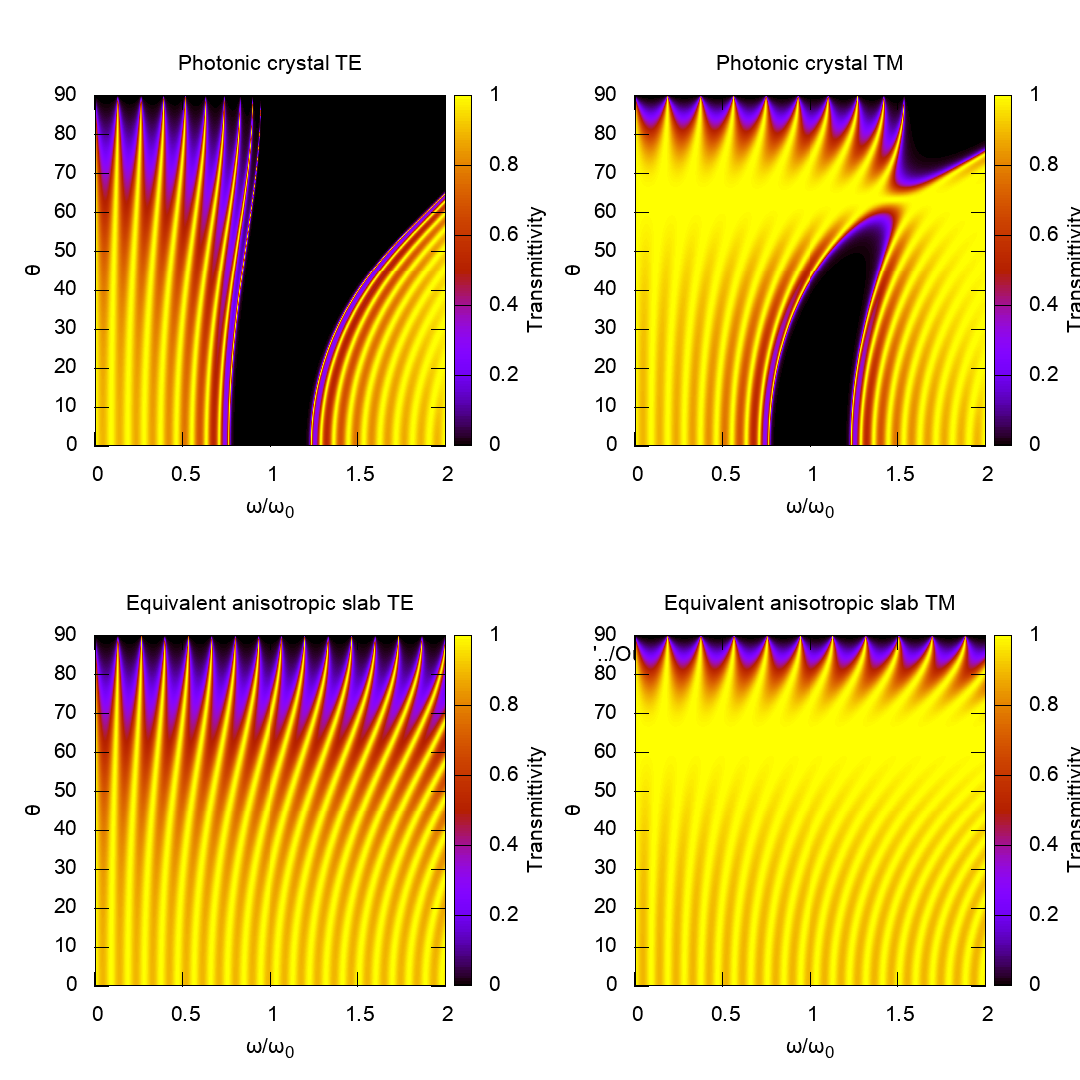
\includegraphics[width=0.85\linewidth]{../Fabry-Perot/Pics/Compare.png}
\end{figure}
\end{document}
